\subsection{Performance comparisons}
As can be seen on \autoref{tab:results-with-many-methods} LightGCN outperforms all the other methods by a significant amount.
With our dataset NGCF performs better than PUP by a small amount, even though Price-Aware recommendation in their paper showcased the opposite \cite{Priceaware}.
Price-Aware recommendation also uses a Yelp dataset for their experiment, however it is not exactly the same dataset.
The results also showcase, that there are a large decrease in performance, when adding prices and categories to the adjacency matrix in LightGCN, which makes it perform worse than any other baseline method.
For NGCF PAS the same changes in input only makes it differentiate negatively by a small amount and actually performs better than PUP.
\begin{table*}[h!]
    \centering
    \begin{tabular}{|l|l|l|l|l|}
        \hline
        \rowcolor[HTML]{FFFFFF}
                       & \multicolumn{4}{l|}{\cellcolor[HTML]{FFFFFF}Yelp Dataset}                                                       \\ \hline
        Method         & Recall@50                                                 & NDCG@50         & Recall@100      & NDCG@100        \\ \hline
        LightGCN       & \textbf{0.2106}                                           & \textbf{0.1063} & \textbf{0.3176} & \textbf{0.1344} \\ \hline
        PUP            & 0.1697                                                    & 0.07802         & 0.2654          & 0.1023          \\ \hline
        GCN            & 0.1558                                                    & 0.07593         & 0.2442          & 0.1001          \\ \hline
        NGCF           & 0.1810                                                    & 0.08817         & 0.2769          & 0.1132          \\ \hline
        GCMC           & 0.1692                                                    & 0.0835          & 0.2497          & 0.1008          \\ \hline
        LGCN PAS (1.0) & 0.1542                                                    & 0.0717          & 0.2199          & 0.086           \\ \hline
        NGCF PAS (1.0) & 0.1749                                                    & 0.0849          & 0.2743          & 0.1111          \\ \hline
    \end{tabular}
    \caption{Results for the experiment with the different methods}
    \label{tab:results-with-many-methods}
\end{table*}
The recall@50 and NDCG@50 for NGCF, NGCF PAS, LightGCN and LGCN PAS can be seen on \autoref{fig:ndcg-50k-lgcn-ngcf-ngcfpas-pas} and \autoref{fig:recall-50k-lgcn-ngcf-ngcfpas-pas}.
Recall@100 and NCDG@100 for the same methods can be seen on \autoref{fig:ndcg-100k-lgcn-ngcf-ngcfpas-pas} and \autoref{fig:recall-100k-lgcn-ngcf-ngcfpas-pas}.
It can be seen that that the difference between the two NGCF graphs are small and only show a small decrease in performance for NGCF PAS.
However for LightGCN and LGCN Pas, there is a large difference.
LGCN has a large decrease in performance, and the graph fluctuates a lot, and does not improve when training.
\begin{figure}
    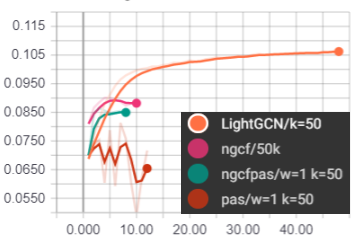
\includegraphics[width=\linewidth]{figures/graphs/ndcg-50k-lgcn-ngcf-ngcfpas-pas.png}
    \caption{NDCG$@$50k on LightGCN, NGCF, NGCF PAS and PAS.}
    \label{fig:ndcg-50k-lgcn-ngcf-ngcfpas-pas}
\end{figure}

\begin{figure}
    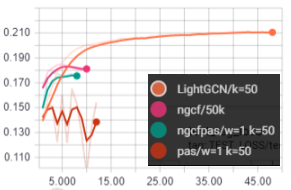
\includegraphics[width=\linewidth]{figures/graphs/recall-50k-lgcn-ngcf-ngcfpas-pas.png}
    \caption{Recall$@$50k on LightGCN, NGCF, NGCF PAS and PAS}
    \label{fig:recall-50k-lgcn-ngcf-ngcfpas-pas}
\end{figure}

\begin{figure}
    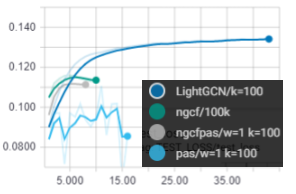
\includegraphics[width=\linewidth]{figures/graphs/ndcg-100k-lgcn-ngcf-ngcfpas-pas.png}
    \caption{NDCG$@$100k on LightGCN, NGCF, NGCF PAS and PAS.}
    \label{fig:ndcg-100k-lgcn-ngcf-ngcfpas-pas}
\end{figure}

\begin{figure}
    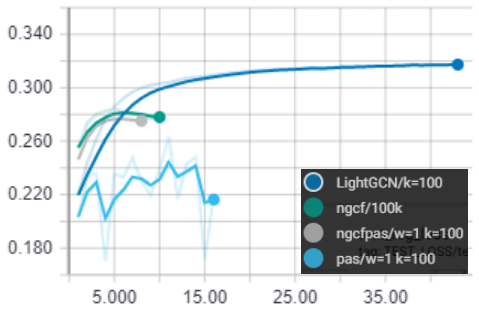
\includegraphics[width=\linewidth]{figures/graphs/recall-100k-lgcn-ngcf-ngcfpas-pas.png}
    \caption{Recall$@$100k on LightGCN, NGCF, NGCF PAS and PAS.}
    \label{fig:recall-100k-lgcn-ngcf-ngcfpas-pas}
\end{figure}


\subsubsection{Hyperparameter experiment}
As described in \autoref{subsec:simple-extension}, we utilize a hyperparameter that is inserted into the adjacency matrix, whenever there is a connection between the item nodes and category nodes, or item nodes and price nodes.
Experiments are done with the hyperparameter $X$ in LGCN PAS and NGCF PAS with the values $0.0$, $0.5$, $1.0$ and $2.0$ to see what effect of this has on the performance.
\begin{table*}[h!]
    \centering
    \begin{tabular}{|l|l|l|l|l|}
        \hline
        \rowcolor[HTML]{FFFFFF}
                       & \multicolumn{4}{l|}{\cellcolor[HTML]{FFFFFF}Yelp Dataset}                                   \\ \hline
        Method         & Recall@50                                                 & NDCG@50 & Recall@100 & NDCG@100 \\ \hline
        LGCN PAS (0.0) & 0.1560                                                    & 0.07674 & 0.2456     & 0.09901  \\ \hline
        LGCN PAS (0.5) & 0.1591                                                    & 0.07825 & 0.2539     & 0.1010   \\ \hline
        LGCN PAS (1.0) & 0.1542                                                    & 0.0717  & 0.2199     & 0.086    \\ \hline
        LGCN PAS (2.0) & 0.1526                                                    & 0.07573 & 0.1581     & 0.06509  \\ \hline
        NGCF PAS (0.0) & 0.1758                                                    & 0.08483 & 0.2737     & 0.1111   \\ \hline
        NGCF PAS (0.5) & 0.1756                                                    & 0.08472 & 0.2744     & 0.1108   \\ \hline
        NGCF PAS (1.0) & 0.1749                                                    & 0.08485 & 0.2743     & 0.1111   \\ \hline
        NGCF PAS (2.0) & 0.1741                                                    & 0.08371 & 0.2762     & 0.1116   \\ \hline
    \end{tabular}
    \caption{Results for the experiment using different input values.}
    \label{tab:hyperparameter-results}
\end{table*}
As can be seen on \autoref{tab:hyperparameter-results} inserting categories and price into the adjacency matrix decreases the performance compared to LightGCN.
The value it has the best performance with is 0.5, followed by 0.0.
Giving prices and categories the same or higher input value as the connection between item and user therefore decreases the results.
On \autoref{fig:ndcg-pas-weights} and \autoref{fig:recall-pas-weights} it can be seen that the graphs fluctuate with the input values that were used.
There could be multiple reasons for this generally not performing well.
The embeddings created from this input could be used, so that it tries to recommend prices and categories, which is not possible.
Another reason could be because LightGCN does not utilize feature transformation and the nonlinear activation function.
LightGCN performs well, if there are only user and item ids, and the decrease in performance could be because LightGCN is unable to handle the semantic representations in price and category.\\
For NGCF changing the input value of price and categories changes almost nothing.
This can also be seen on \autoref{fig:ndcg-pas-weights} and \autoref{fig:recall-ngcfpas-weights}.
This is likely because the embeddings for price and categories are never used.
However, we did have an initial idea, that the convolutions with price and category would be reflected onto users and items, which is seen to give a very minimal effect on the outcome.


\begin{figure}
    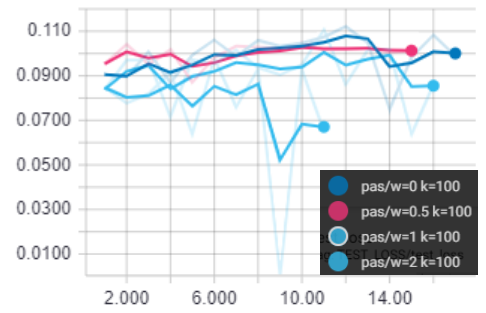
\includegraphics[width=\linewidth]{figures/graphs/ndcg-pas-weights.png}
    \caption{NDCG$@$100 on PAS with different input values}
    \label{fig:ndcg-pas-weights}
\end{figure}

\begin{figure}
    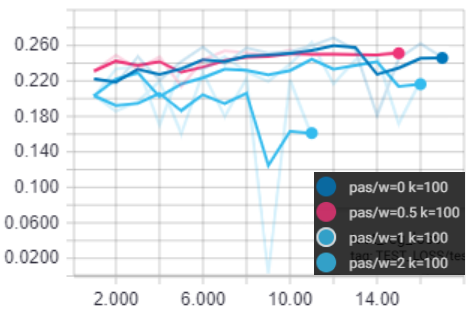
\includegraphics[width=\linewidth]{figures/graphs/recall-pas-weights.png}
    \caption{Recall$@$100k on PAS with different input values}
    \label{fig:recall-pas-weights}
\end{figure}

\begin{figure}
    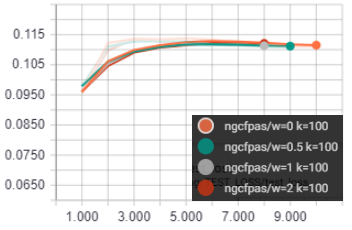
\includegraphics[width=\linewidth]{figures/graphs/ndcg100-ngcfpas-weights.png}
    \caption{NDCG$@$100k on NGCF PAS with different input values}
    \label{fig:ndcg-ngcfpas-weights}
\end{figure}

\begin{figure}
    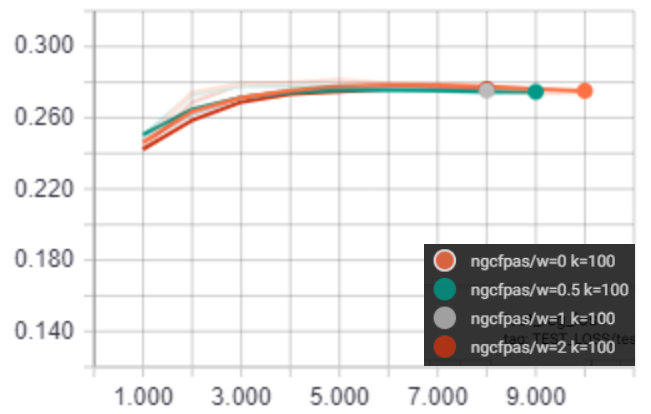
\includegraphics[width=\linewidth]{figures/graphs/recall-ngcfpas-weights.png}
    \caption{Recall$@$100k on NGCF PAS with different input values}
    \label{fig:recall-ngcfpas-weights}
\end{figure}
